\chapter{Results}
\label{chap:experiments}

\ifdraftresults
\begin{quote}
\textbf{Preliminary development results---not for final comparison.}
The values in this chapter come from the reduced workflow used to test data
collection and report generation.  Meshes, final times, repetitions, and the
experiment matrix have not yet been approved for the thesis-final study.  The
figures and tables demonstrate presentation style only and must not be cited as
final numerical evidence.
\end{quote}

\section{Convergence-table convention}
\label{sec:results-convergence-tables}

For the periodic one-dimensional advection problem, define
\begin{align}
 e_1&=\|u-u_h\|_{L^1(\Omega)},\\
 e_2&=\|u-u_h\|_{L^2(\Omega)},\\
 e_3&=\|u-u_h\|_{L^\infty(\Omega)},\\
 e_4&=\left(h\sum_j\left|
      \frac1h\int_{I_j}(u-u_h)\,\mathrm dx\right|^2\right)^{1/2},\\
 e_5&=\left(h\sum_j\left|
      u(x_{j+1/2})-u_h(x_{j+1/2}^-)\right|^2\right)^{1/2}.
 \label{eq:five-advection-errors}
\end{align}
The first three errors measure the full polynomial solution.  The latter two
measure cell-average and downwind-point superconvergence after Gauss--Radau
initialization.  Each method receives a separate table with identical degree
and mesh rows.  A missing first rate is written as ``--'' rather than assigned
a numerical value.

\IfFileExists{generated/draft/tables/advection_1d_dg.tex}{
  % Generated by scripts/analyze_study.py; do not edit.
\begin{table}[htbp]
\centering
\small
\setlength{\tabcolsep}{3.0pt}
\caption{Preliminary development run: errors and convergence rates for RKDG on smooth one-dimensional advection.}
\label{tab:advection-dg}
\begin{tabular}{c r rr rr rr rr rr}
\toprule
$k$ & $N_x$ & $e_1$ & rate & $e_2$ & rate & $e_3$ & rate & $e_4$ & rate & $e_5$ & rate \\
\midrule
\multirow{3}{*}{1} & 20 & 7.04e-03 & -- & 8.26e-03 & -- & 1.58e-02 & -- & 1.35e-03 & -- & 1.78e-03 & -- \\
 & 40 & 1.77e-03 & 1.99 & 2.11e-03 & 1.97 & 4.47e-03 & 1.82 & 1.81e-04 & 2.90 & 2.36e-04 & 2.92 \\
 & 80 & 4.36e-04 & 2.02 & 5.30e-04 & 1.99 & 1.17e-03 & 1.94 & 2.34e-05 & 2.96 & 3.01e-05 & 2.97 \\
\midrule
\multirow{3}{*}{2} & 20 & 3.28e-04 & -- & 4.26e-04 & -- & 9.33e-04 & -- & 7.19e-06 & -- & 1.07e-05 & -- \\
 & 40 & 4.00e-05 & 3.04 & 5.35e-05 & 2.99 & 1.18e-04 & 2.98 & 2.35e-07 & 4.94 & 3.50e-07 & 4.93 \\
 & 80 & 4.96e-06 & 3.01 & 6.69e-06 & 3.00 & 1.48e-05 & 3.00 & 7.46e-09 & 4.98 & 1.10e-08 & 4.99 \\
\bottomrule
\end{tabular}
\end{table}

  % Generated by scripts/analyze_study.py; do not edit.
\begin{table}[htbp]
\centering
\small
\setlength{\tabcolsep}{3.0pt}
\caption{Preliminary development run: errors and convergence rates for adapted OFDG--KXRCF on smooth one-dimensional advection.}
\label{tab:advection-ofdg-kxrcf}
\begin{tabular}{c r rr rr rr rr rr}
\toprule
$k$ & $N_x$ & $e_1$ & rate & $e_2$ & rate & $e_3$ & rate & $e_4$ & rate & $e_5$ & rate \\
\midrule
\multirow{3}{*}{1} & 20 & 1.37e-02 & -- & 1.76e-02 & -- & 3.18e-02 & -- & 1.28e-02 & -- & 1.90e-02 & -- \\
 & 40 & 2.62e-03 & 2.39 & 3.24e-03 & 2.44 & 7.71e-03 & 2.04 & 2.25e-03 & 2.50 & 2.71e-03 & 2.81 \\
 & 80 & 5.27e-04 & 2.31 & 6.55e-04 & 2.30 & 2.18e-03 & 1.82 & 3.64e-04 & 2.63 & 4.12e-04 & 2.72 \\
\midrule
\multirow{3}{*}{2} & 20 & 6.90e-04 & -- & 9.73e-04 & -- & 2.18e-03 & -- & 8.00e-04 & -- & 9.00e-04 & -- \\
 & 40 & 4.47e-05 & 3.95 & 5.82e-05 & 4.06 & 1.57e-04 & 3.80 & 2.13e-05 & 5.23 & 1.63e-05 & 5.79 \\
 & 80 & 4.99e-06 & 3.16 & 6.69e-06 & 3.12 & 1.48e-05 & 3.41 & 2.06e-07 & 6.69 & 3.70e-07 & 5.46 \\
\bottomrule
\end{tabular}
\end{table}

  % Generated by scripts/analyze_study.py; do not edit.
\begin{table}[htbp]
\centering
\small
\setlength{\tabcolsep}{3.0pt}
\caption{Preliminary development run: errors and convergence rates for 2024 OEDG on smooth one-dimensional advection.}
\label{tab:advection-oedg}
\begin{tabular}{c r rr rr rr rr rr}
\toprule
$k$ & $N_x$ & $e_1$ & rate & $e_2$ & rate & $e_3$ & rate & $e_4$ & rate & $e_5$ & rate \\
\midrule
\multirow{3}{*}{1} & 20 & 1.47e-02 & -- & 1.80e-02 & -- & 3.15e-02 & -- & 1.44e-02 & -- & 1.76e-02 & -- \\
 & 40 & 2.89e-03 & 2.34 & 3.52e-03 & 2.36 & 6.54e-03 & 2.27 & 2.66e-03 & 2.44 & 3.02e-03 & 2.55 \\
 & 80 & 5.84e-04 & 2.31 & 6.74e-04 & 2.39 & 1.15e-03 & 2.50 & 4.03e-04 & 2.72 & 4.39e-04 & 2.78 \\
\midrule
\multirow{3}{*}{2} & 20 & 1.05e-03 & -- & 1.25e-03 & -- & 2.85e-03 & -- & 1.01e-03 & -- & 1.30e-03 & -- \\
 & 40 & 6.68e-05 & 3.97 & 8.47e-05 & 3.88 & 2.01e-04 & 3.83 & 5.37e-05 & 4.23 & 6.45e-05 & 4.33 \\
 & 80 & 6.12e-06 & 3.45 & 7.85e-06 & 3.43 & 1.83e-05 & 3.46 & 2.84e-06 & 4.24 & 3.37e-06 & 4.26 \\
\bottomrule
\end{tabular}
\end{table}

}{
  The draft convergence tables are generated by
  \texttt{make figures-draft} from the reduced checkpoint.
}

\section{Smooth accuracy presentation}

Convergence curves are separated by polynomial degree so that an axis contains
only the three headline methods and one reference slope.  Complete values
remain in the corresponding paper-style tables.

\IfFileExists{generated/draft/figures/convergence_advection_1d_p1.pdf}{
\begin{figure}[htbp]
  \centering
  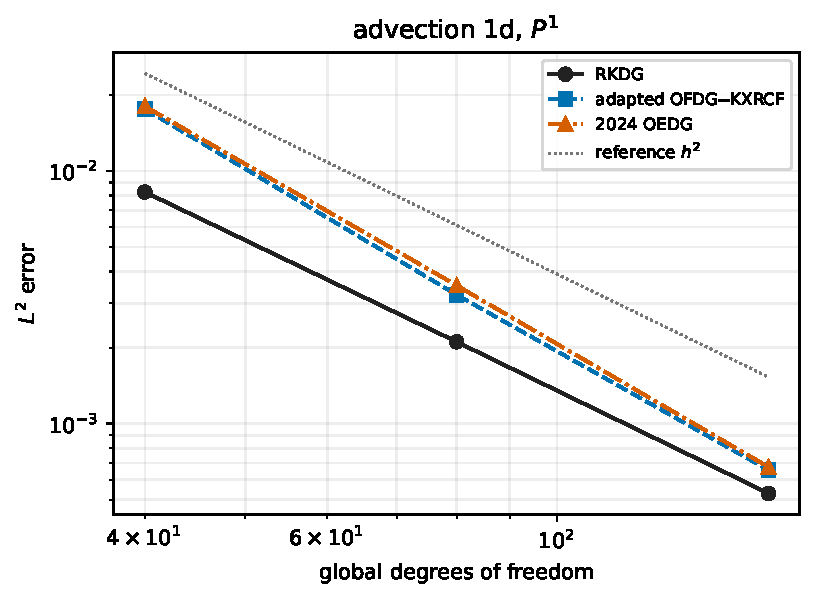
\includegraphics[width=.74\textwidth]{generated/draft/figures/convergence_advection_1d_p1.pdf}
  \caption{Preliminary development run for periodic 1D advection with $P^1$
  elements.  The plot compares $L^2$ error against actual global degrees of
  freedom for the three headline methods; the dotted line is the expected
  second-order slope.  These values are not part of the final study.}
  \label{fig:draft-advection-p1}
\end{figure}

\begin{figure}[htbp]
  \centering
  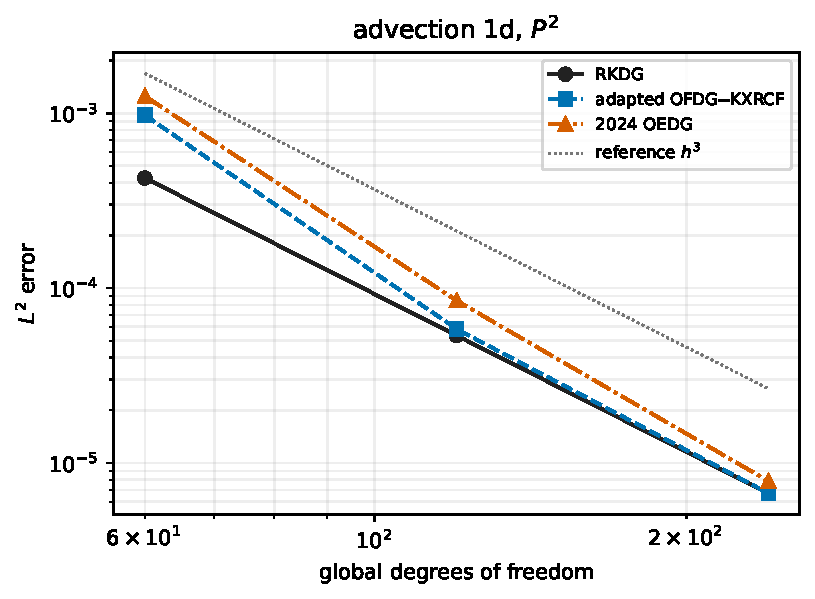
\includegraphics[width=.74\textwidth]{generated/draft/figures/convergence_advection_1d_p2.pdf}
  \caption{Preliminary development run for periodic 1D advection with $P^2$
  elements.  The plot compares $L^2$ error against actual global degrees of
  freedom for the three headline methods; the dotted line is the expected
  third-order slope.  These values are not part of the final study.}
  \label{fig:draft-advection-p2}
\end{figure}
}{ }

\section{Discontinuity and invariance presentation}

One-dimensional discontinuity figures show at most the three headline methods
and the independent reference.  A matched inset is retained only when it
reveals a steep-gradient difference that is not visible in the full-domain
view.  Scale-invariance figures use one panel per method and compare normalized
solutions at fixed numerical settings.

\IfFileExists{generated/draft/figures/profile_lax_scaled_p2.pdf}{
\begin{figure}[htbp]
  \centering
  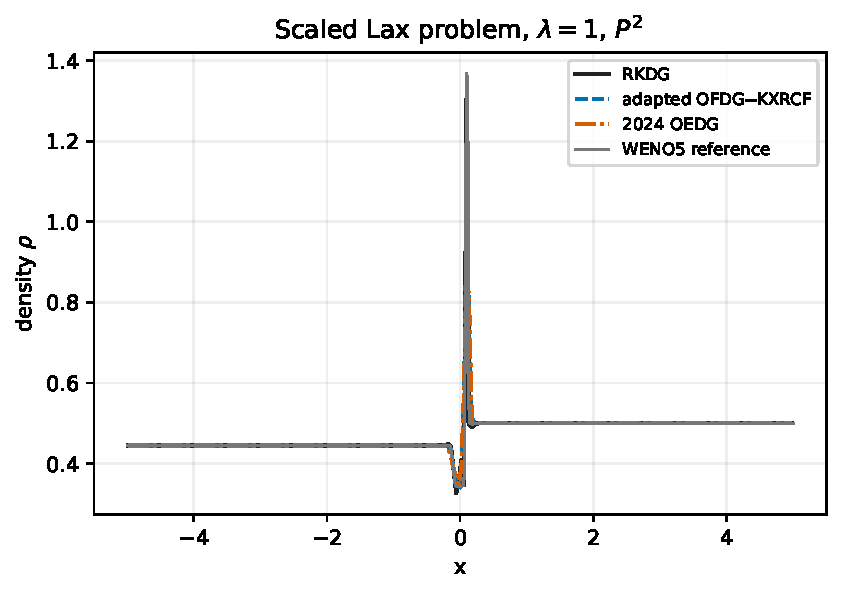
\includegraphics[width=.76\textwidth]{generated/draft/figures/profile_lax_scaled_p2.pdf}
  \caption{Preliminary development profile for scaled Lax data with $P^2$
  elements at the reduced final time.  Density is compared with the independent
  WENO5 reference.  These values are not part of the final study.}
  \label{fig:draft-lax-profile}
\end{figure}

\begin{figure}[htbp]
  \centering
  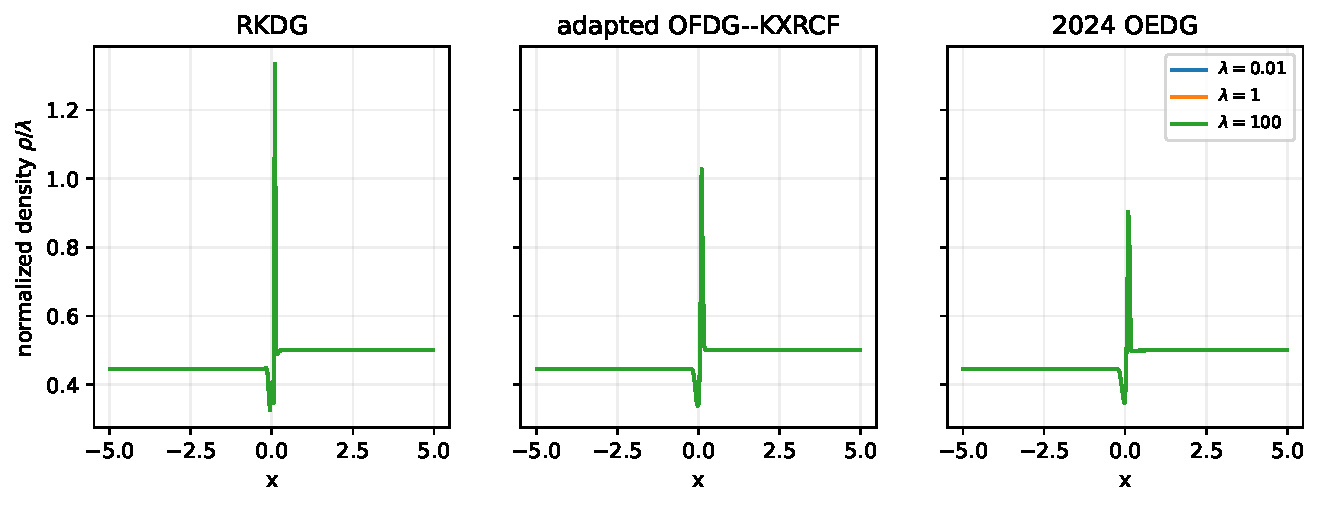
\includegraphics[width=.95\textwidth]{generated/draft/figures/scale_invariance_p2.pdf}
  \caption{Preliminary normalized-density presentation for the three proposed
  Lax scales with $P^2$ elements.  Each panel contains one method, so coincident
  curves directly test scale invariance without mixing methods.  These values
  are not part of the final study.}
  \label{fig:draft-scale-invariance}
\end{figure}
}{ }

\section{Two-dimensional presentation}

Contour comparisons and line cuts are deliberately separated.  The contour
figure uses identical limits and levels for all methods; the line-cut figure
then has sufficient width for direct quantitative comparison.

\IfFileExists{generated/draft/figures/contour_riemann_2d_p1.pdf}{
\begin{figure}[htbp]
  \centering
  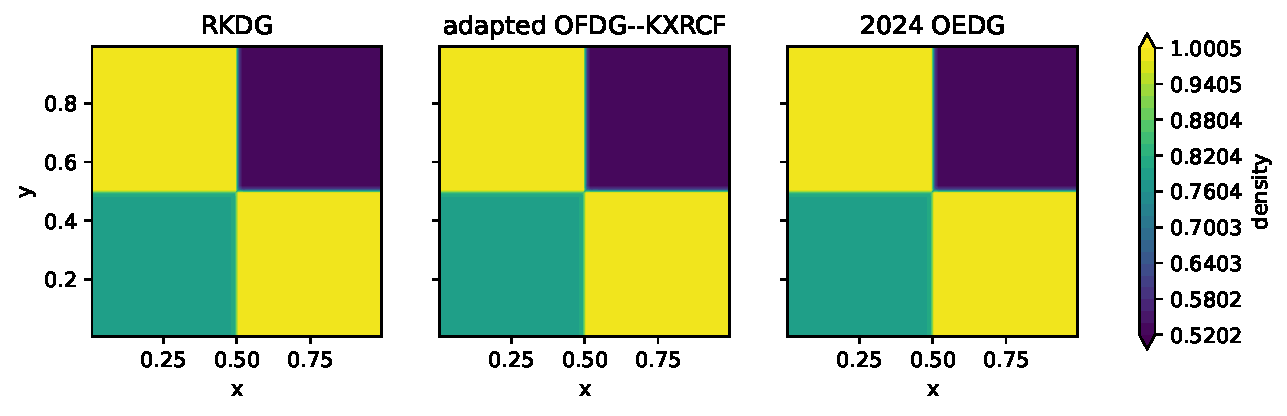
\includegraphics[width=.98\textwidth]{generated/draft/figures/contour_riemann_2d_p1.pdf}
  \caption{Preliminary development density contours for the reduced two-rank
  2D Riemann problem with $P^1$ elements.  Identical contour levels are used
  for all headline methods.  These values are not part of the final study.}
  \label{fig:draft-riemann-contours}
\end{figure}

\begin{figure}[htbp]
  \centering
  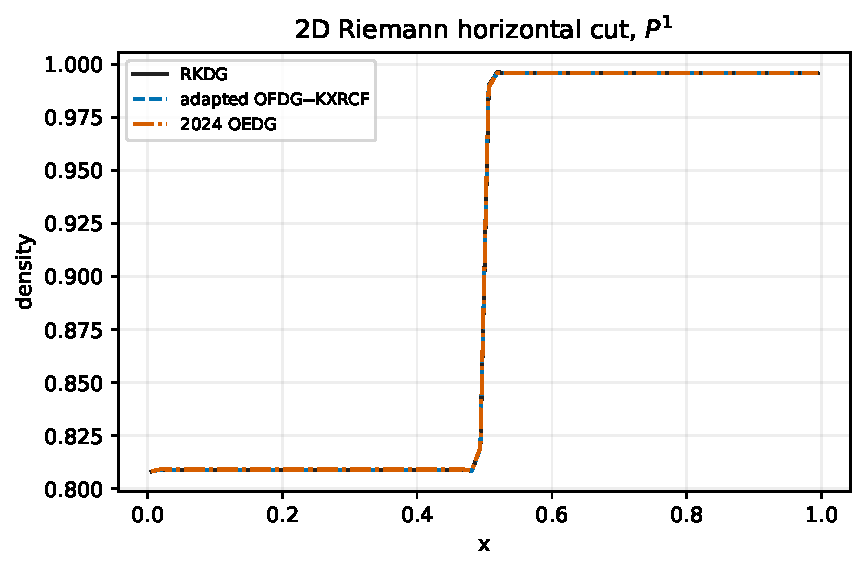
\includegraphics[width=.78\textwidth]{generated/draft/figures/linecut_riemann_2d_p1.pdf}
  \caption{Horizontal density cuts corresponding to
  \cref{fig:draft-riemann-contours}.  The sampling convention is identical for
  all methods.  These values are not part of the final study.}
  \label{fig:draft-riemann-linecuts}
\end{figure}
}{ }

\section{Detector, robustness, and cost presentation}

The final KXRCF result will show indicator values, the threshold, and active
cells along the same spatial coordinate as a representative shock profile.
The reduced checkpoint did not record spatial indicator values, so no surrogate
activation chart is shown here.  Positivity activity and unassisted failure
times will be tabulated rather than compressed into a many-category bar chart.
Runtime plots will be problem- and degree-specific and will use repeated timing
rows only; the single-run development timings are deliberately omitted.

\else
\InputIfFileExists{generated/final/results.tex}{}{%
  \PackageError{thesis}{Approved final results are missing}{Run the guarded
  final study and analysis before building report-final.}}
\fi
